%\input{sections/martian-environment/references.tex}

\section{Seasons}
\label{sec:MartianEnvironment:Seasons}
The red planet's axis is tilted away from the sun at \SI{25}{\degree}. Very much like Earth's \SI{23.5}{\degree} axial tilt, this results in seasons. Mars has an orbit with a semi-major axis of \SI{1.524}{\astronomicalunit} which translates to a Martian year corresponding to an orbital period of 687 days. Martian seasons are longer and for every Martian year 1.88 Earth years go by. Sidereal days are 24.62 hours long and solar days are 24.65 hours long. A Martian day, known as a Sol, is approximately 40 minutes longer than an Earth day. Mars' position on its orbit is described in terms of areocentric longitude of the Sun, $L_{s}$, and is measured Eastwards from $L_{s}$ = \SI{0}{\degree} at the northern hemisphere's Vernal equinox. The transition of Martian seasons are presented in Table \ref{table:mars-seasonal-advances} with respect to areocentric longitudes.

\begin{table}[H]
  \centering
  \caption{Seasonal advances on Mars.}
  \label{tab:mars-seasonal-advances}
  \begin{tabular}{|l|l|l|}
  \hline
  \multirow{2}{*}{\textbf{\begin{tabular}[c]{@{}l@{}}Areocentric\\ Longitude\end{tabular}}} & \multicolumn{2}{c|}{\textbf{Seasonal Advance}} \\ \cline{2-3}
   & \multicolumn{1}{c|}{\textbf{Northern Hemisphere}} & \multicolumn{1}{c|}{\textbf{Southern Hemisphere}} \\ \hline
  \textbf{\si{0}{\degree}} & Vernal Equinox & Autumnal Equinox \\ \hline
  \textbf{\si{0}{\degree} to \si{90}{\degree}} & Spring & Autumn \\ \hline
  \textbf{\si{90}{\degree}} & Summer Solstice & Winter Solstice \\ \hline
  \textbf{\si{90}{\degree} to \si{180}{\degree}} & Summer & Winter \\ \hline
  \textbf{\si{180}{\degree}} & Autumnal Equinox & Vernal Equinox \\ \hline
  \textbf{\si{180}{\degree} to \si{270}{\degree}} & Autumn & Spring \\ \hline
  \textbf{\si{270}{\degree}} & Winter Solstice & Summer Solstice \\ \hline
  \textbf{\si{270}{\degree} to \si{360}{\degree}} & Winter & Summer \\ \hline
  \end{tabular}
\end{table}



\section{Dust Storms}
\label{sec:MartianEnvironment:DustStorms}

The great fluctuations in temperature and the difference in warmth between hemispheres can cause huge dust storms. Some can affect just a small area, while others can cover the entire planet. The larger storms usually occur when the planet is near its aphelion (closest point to the Sun). When there are global dust storms there is no way for scientists to visualize the planet’s surface.

Great dust storms (area > 10e6 km2) occur with a yearly probability of 30\% to 80\%. \citepower{Kerslake1999}

Local dust storms (area < 10e6 km2) occur with a 5\% probability in Mars equatorial regions and have only a minor impact on seasonal insulation due to their limited size, duration (a few days), and moderate OD (~1). \citepower{Kerslake1999}

the dust accumulation rate is assumed to be 5\% of that measured by Pathfinder \citepower{Kerslake1999}

Losses from lander vehicle shadowing and terrain masking are not yet modeled pending better definitions of lander configuration and landing sites. \citepower{Kerslake1999}

For desirable near-equatorial landing sites (not in canyons), shadowing and terrain masking losses will be small. This is due to high sun angles (that create short shadows) and the large component of diffuse solar insolation near dusk and dawn (when the terrain masking effect is largest). \citepower{Kerslake1999}

\section{Solar Radiation}
\label{sec:MartianEnvironment:SolarRadiation}
%\input{sections/s.tex}

% Martian Season - start with images
% Regolith, dust, and craters, other elements
% Settle with locations DTM
Solar radiation calculations presented in this section as well as nomenclatures are taken from \citemarsenv{Appelbaum1990}.

\subsection{Irradiance}

Beam irradiance, expressed in \SI{}{\watt\meter\squared}, is a measure of solar radiation from direct sunlight. At the top of the Martian atmosphere the instantaneous beam irradiance is a function of areocentric longitude, expressed as $G_{ob}$, as shown in Equation \ref{eq:G_ob}.

\begin{equation}
  \label{eq:G_ob}
  G_{ob} = 590 \frac{[1 + e \cos{(Ls - 248)}]^2}{(1-e^2)^2}
\end{equation}

Where \SI{590}{\watt\meter\squared} is the mean beam irradiance at the top of the Martian atmosphere, $L_{s}$ - \SI{248}{\degree} is the true anomaly, and e is the Mars eccentricity. The variation of $G_{ob}$ is presented in Figure \ref{fig:plot:beam-irradiance-top-of-mars-atmosphere}.

\begin{figure}[H]%[b]
%\vspace{-2ex}
  \centering
  \hypersetup{linkcolor=captionTextColor}
  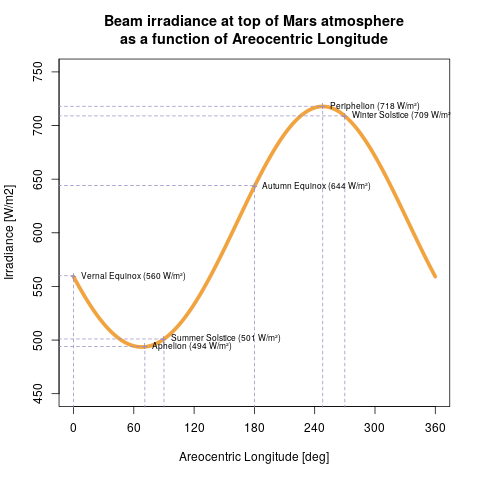
\includegraphics[width=0.8\linewidth]{sections/martian-environment/plots/beam-irradiance-at-top-of-mars-atmosphere-as-a-function-of-areocentric-longitude.png}\\
  %\vspace{-2ex}
  \caption[Beam irradiance at top of Mars atmosphere as a function of Areocentric Longitude]
          {Beam irradiance at top of Mars atmosphere as a function of Areocentric Longitude}
  \label{fig:plot:beam-irradiance-top-of-mars-atmosphere}
  %\vspace{-3ex}
\end{figure}

At its closest, the periphelion, Mars is at a distance of \SI{1.381}{\astronomicalunit} from the sun with a beam irradiance on top of its atmosphere reaching its maximum of \SI{718}{\watt\meter\squared} at $L_{s} = \SI{248}{\degree}$. At its furthest of \SI{1.666}{\astronomicalunit}, the aphelion, the beam irradiance reaches its minimum of \SI{494}{\watt\meter\squared} at $L_{s} = \SI{71}{\degree}$.

Further parameterization becomes necessary in order to measure beam irradiance on a horizontal surface at the top Mars atmosphere where the solar zenith angle $z$, must be considered. The solar zenith angle itself is a function of planetary latitude $\phi$, declination angle $\delta$, and hour angle $\omega$ measured from the true noon westward. Expressed as $G_{obh}$ from \citemarsenv{Appelbaum1990}:

\begin{equation}
  \label{eq:G_obh}
  G_{obh} = G_{ob}\cos{z}
\end{equation}

Where z is given by:

\begin{equation}
  \label{eq:cosz}
  \cos{z} = \sin{\phi}\sin{\delta} + \cos{\phi}\cos{\delta}\cos{\omega}
\end{equation}

Examples of solar radiation calculations using Equation \ref{eq:G_obh} as a function of Solar Time can be found in \citemarsenv{Appelbaum1990} for Viking Lander VL1 at various points of $L_s$. By way of example, equivalent calculations at MER Opportuny's final resting location at Endeavour crater are presented in Figure \ref{fig:plot:diurnal-variation-of-beam-irradiance-on-a-horizontal-surface-at-top-of-mars-atmosphere}.

\begin{figure}[H]
  \centering
  \hypersetup{linkcolor=captionTextColor}
  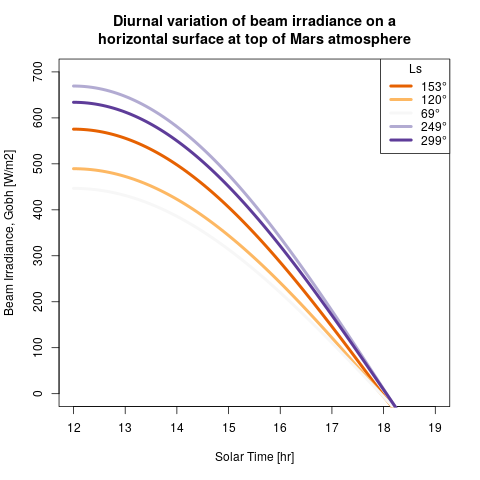
\includegraphics[width=0.8\linewidth]{sections/martian-environment/plots/diurnal-variation-of-beam-irradiance-on-a-horizontal-surface-at-top-of-mars-atmosphere.png}\\
  \caption[Diurnal variation of beam irradiance on a horizontal surface at top of Mars atmosphere]
  {Diurnal variation of beam irradiance on a horizontal surface at top of Mars atmosphere}
  \label{fig:plot:diurnal-variation-of-beam-irradiance-on-a-horizontal-surface-at-top-of-mars-atmosphere}
\end{figure}

% Mention that we want diurnal plots of irradiance so best to use solar time...
% Now we want to express in time.

Obtaining the irradiance on the surface of Mars requires the atmospheric opacity as an additional parameter. A distinction exists between global, direct, and diffuse beam irradiance where global beam irradiance $G_{h}$ is the sum of direct, $G_{bh}$, and diffuse beam irradiances, $G_{dh}$:

\begin{equation}
  \label{eq:G_h_1}
  G_{h} = G_{bh} + G_{dh}
\end{equation}

The expression for $G_{h}$ and $G_{bh}$ are presented in Equations \ref{eq:G_h} and \ref{eq:G_bh}, taken from \citemarsenv{Appelbaum1990}:

\begin{equation}
  \label{eq:G_h_2}
  G_{h} = G_{ob}\cos{z}\frac{f(z,\tau)}{0.9}
\end{equation}

Where $f(z,\tau)$ is the normalized net flux function derived from the net solar flux integrated over the solar spectrum on the Martian surface and 0.9 comes from the $(1-albedo)$ expression for an albedo of 0.1 \citemarsenv{Appelbaum1990}.

\begin{equation}
  \label{eq:G_bh}
  G_{bh} = G_{ob}\cos{z}\exp(\frac{-\tau}{cos{z}})
\end{equation}

Diurnal irradiance profiles are presented in Figure \ref{} for different planetary latitudes during the periphelion.

\subsection{Insolation}

Solar insolation is the amount solar radiation incident on a planetary surface during a time period. It is expressed in \si{\watt\hour\per\meter\squared} and obtained by integrating the equations of irradiance over a time period between $\omega_1$ and $\omega_2$. Thus, insolation on a horizontal surface at the top of Mars atmosphere, denoted as $I_{obh}$, is obtained by integrating Equation \ref{eq:G_h_2} of $G_{obh}$.

Global, beam, and diffuse insolations on a horizontal Mars surface are denoted as $I_{h}$, $I_{bh}$, and $I_{dh}$ respectively. Their values are obtained by integrating \ref{eq:G_h_2} for $I_{h}$ and \ref{eq:G_bh} for $I_{bh}$. Diffuse insolation $I_{dh}$ is obtained through the same relationship presented in Equation \ref{eq:G_h_1}. The variation of insolation as a function of $L_{s}$ for different levels of atmospheric opacities are illustrated in Figure \ref{fig:insolation-ls} with MER Opportunity's final location. Evidently, the insolation curves peak at the periphelion with $L_{s} = \SI{248}{\degree}$ and reach their lowest during the aphelion with $L_{s} = \SI{71}{\degree}$. Interestingly, diffuse insolation is already the largest component contributing to the global insolation at $\tau = 1$ and, on a dusty day at $\tau = 3$, global insolation is mostly diffuse.

\begin{figure}[H]
\vspace{-2ex}
	\centering
    %% setup sizes
    \setlength{\subfigureWidth}{0.50\textwidth}
    \setlength{\graphicsHeight}{80mm}
    %% kill hyper-link highlighting
    \hypersetup{hidelinks=true}%
    %% the figures
%% 1st row
  	\begin{subfigure}[t]{\subfigureWidth}
      \centering
  		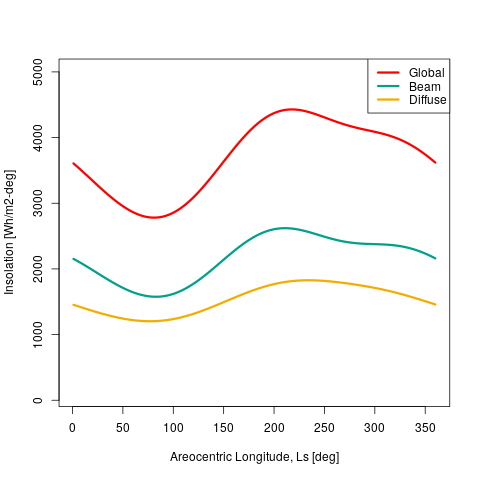
\includegraphics[height=\graphicsHeight]{sections/martian-environment/plots/variation-of-global-beam-and-diffuse-insolation-on-mars-horizontal-surface-as-a-function-of-areocentric-longitude-for-tau05-and-phi205.png}
  		\subcaption{Tau factor 0.5}
  		\label{fig:sub:insolation-ls-tau-factor-0p5}
  	\end{subfigure}\hfill
    \begin{subfigure}[t]{\subfigureWidth}
      \centering
  		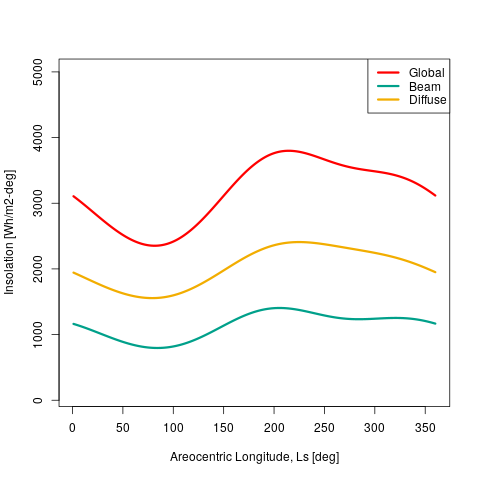
\includegraphics[height=\graphicsHeight]{sections/martian-environment/plots/variation-of-global-beam-and-diffuse-insolation-on-mars-horizontal-surface-as-a-function-of-areocentric-longitude-for-tau1-and-phi205.png}
  		\subcaption{Tau factor 1}
  		\label{fig:sub:insolation-ls-tau-factor-1}
  	\end{subfigure}\\[0.8ex]
%% 2nd row
    \begin{subfigure}[t]{\subfigureWidth}
      \centering
  		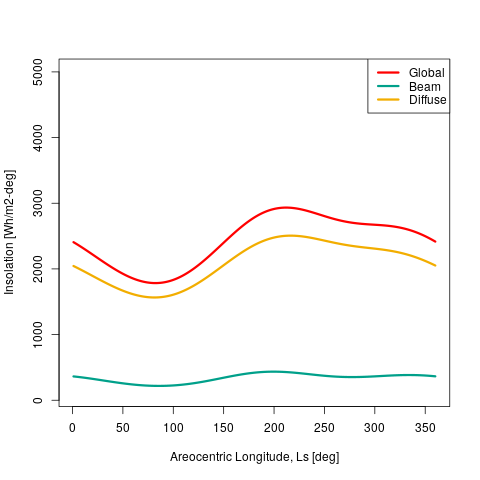
\includegraphics[height=\graphicsHeight]{sections/martian-environment/plots/variation-of-global-beam-and-diffuse-insolation-on-mars-horizontal-surface-as-a-function-of-areocentric-longitude-for-tau2-and-phi205.png}
  		\subcaption{Tau factor 2}
  		\label{fig:sub:insolation-ls-tau-factor-2}
  	\end{subfigure}\hfill
	   \begin{subfigure}[t]{\subfigureWidth}
      \centering
  		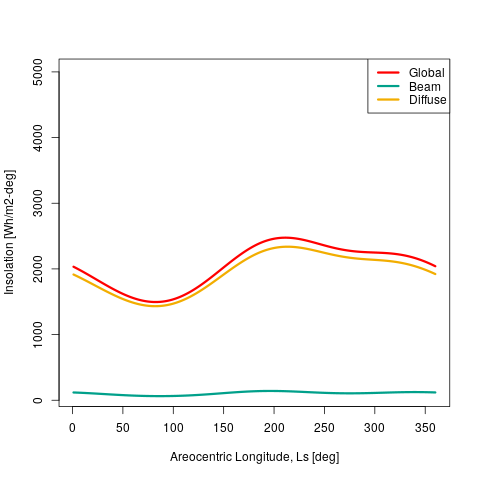
\includegraphics[height=\graphicsHeight]{sections/martian-environment/plots/variation-of-global-beam-and-diffuse-insolation-on-mars-horizontal-surface-as-a-function-of-areocentric-longitude-for-tau3-and-phi205.png}
  		\subcaption{Tau factor 3}
  		\label{fig:sub:insolation-ls-tau-factor-3}
	   \end{subfigure}\hfill
	\caption{Variation of global, beam, and diffuse insolation on Mars horizontal surface as a function of areocentric longitude.}
	\label{fig:insolation-ls}
\vspace{-2ex}
\end{figure}

Daily insolations are obtained when $\omega_1$ and $\omega_2$ are set for a time period between sunrise and sunset. The resulting values are denoted as $H_{h}$, $H_{bh}$, and $H_{dh}$ for global, beam, and diffuse insolations on Mars horizontal surface and $H_{obh}$ for a horizontal surface at the top of Mars atmosphere. Similarly to $I_{dh}$, the daily diffuse insolations $H_{dh}$ is obtained from the same relationship presented in Equation \ref{eq:G_h_1}.

To illustrate the variation of beam, direct, and diffuse insolations during a Martian day, a diurnal profile is presented in Figure \ref{fig:insolation-phi} at different planetary latitudes during the aphelion for a clear day with $\tau = 0.5$. The seasonal influences are evident: at $L_{s} = \SI{71}{\degree}$, it is Autumn in the northern hemisphere and insolations at $\phi = \SI{20}{\degree}$ are much greater than those in the southern hemisphere at $\phi = \SI{-20}{\degree}$ and $\phi = \SI{-40}{\degree}$. Furthermore, daylight at $\phi = \SI{20}{\degree}$ spans across 16 hours whereas it only lasts for 12 hours at $\phi = \SI{-20}{\degree}$ and 10 hours at $\phi = \SI{-40}{\degree}$ .


\begin{figure}[H]
\vspace{-2ex}
	\centering
    %% setup sizes
    \setlength{\subfigureWidth}{0.50\textwidth}
    \setlength{\graphicsHeight}{80mm}
    %% kill hyper-link highlighting
    \hypersetup{hidelinks=true}%
    %% the figures
%% 1st row
  	\begin{subfigure}[t]{\subfigureWidth}
      \centering
  		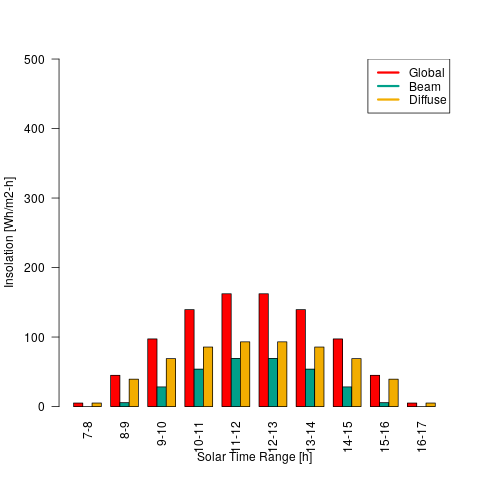
\includegraphics[height=\graphicsHeight]{sections/martian-environment/plots/diurnal-insolation-variation-1-for-ls-71-phi-40-and-tau-05.png}
  		\subcaption{$\phi = \SI{-40}{\degree}$}
  		\label{fig:sub:insolation-phi-m40}
  	\end{subfigure}\hfill
    \begin{subfigure}[t]{\subfigureWidth}
      \centering
  		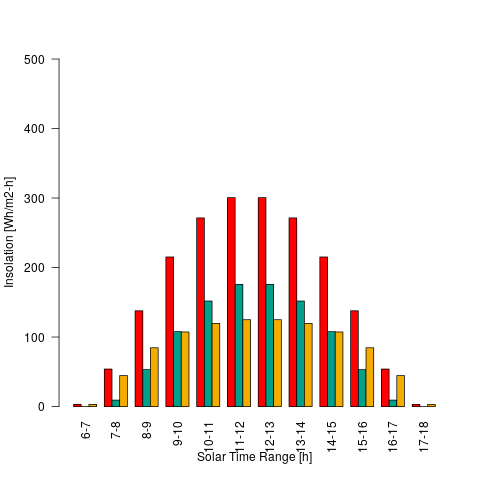
\includegraphics[height=\graphicsHeight]{sections/martian-environment/plots/diurnal-insolation-variation-2-for-ls-71-phi-20-and-tau-05.png}
  		\subcaption{$\phi = \SI{-20}{\degree}$}
  		\label{fig:sub:insolation-phi-m20}
  	\end{subfigure}\\[0.8ex]
%% 2nd row
    \begin{subfigure}[t]{\subfigureWidth}
      \centering
  		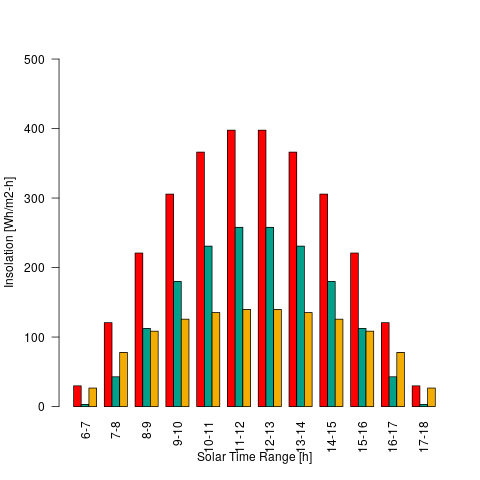
\includegraphics[height=\graphicsHeight]{sections/martian-environment/plots/diurnal-insolation-variation-3-for-ls-71-phi-0-and-tau-05.png}
  		\subcaption{$\phi = \SI{0}{\degree}$}
  		\label{fig:sub:insolation-phi-0}
  	\end{subfigure}\hfill
	   \begin{subfigure}[t]{\subfigureWidth}
      \centering
  		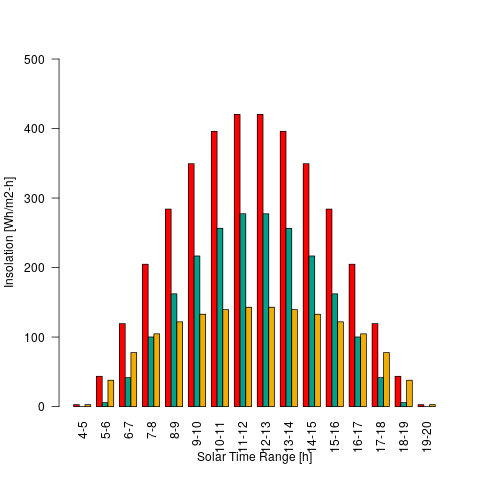
\includegraphics[height=\graphicsHeight]{sections/martian-environment/plots/diurnal-insolation-variation-4-for-ls-71-phi-40-and-tau-05.png}
  		\subcaption{$\phi = \SI{20}{\degree}$}
  		\label{fig:sub:insolation-phi-p20}
	   \end{subfigure}\hfill
	\caption{Diurnal variation global, beam, and diffuse insolation on Mars horizontal surface at different planetary latitudes.}
	\label{fig:insolation-phi}
\vspace{-2ex}
\end{figure}


\section{Dust Storms}
\label{sec:MartianEnvironment:DustStorms}
%\input{sections/s.tex}
